\subsection{The Planner}
\label{sec:voronoiplanner}

Our planner is \emph{reactive} in the sense that it does not remember its past inputs or outputs.
The input is simply a 2D point-cloud from lidar, and the output is a 2D \emph{waypoint} passed to the controller.
We assume that the environment is polygonal.
% Basically, t
The planner calculates a Voronoi diagram corresponding to the point-cloud, then it chooses a point on the Voronoi diagram as the waypoint.

The first step is to calculate a Voronoi diagram.
Since the environment is polygonal, the planner converts the 2D point cloud to a set of line segments based on co-linearity and connectivity thresholds.
\emph{Co-linearity threshold} determines the minimum angle between consecutive line segments of a polyline.
\emph{Connectivity threshold} determines the minimum distance between two co-linear line segments.
Representing a set of points by a line segment simplifies the computation and representation of the Voronoi diagram.
Since the input to the Voronoi computation is a set of line segments, the Voronoi edges are either linear or parabolic arcs.
After computing the Voronoi diagram, we approximate each parabolic edge by a polyline using a \emph{deviation threshold}.
The \emph{deviation threshold} determines the maximum distance of the points on a parabolic arc from the approximating polyline.
This linear approximation simplifies the planner and its formal analysis.
A Voronoi diagram calculated by the planner is called a \emph{local} Voronoi diagram since it is computed for the point-cloud visible from lidar.
This is in contrast to the \emph{global} Voronoi diagram where the diagram is computed with respect to the whole polygonal environment (which is not available to the car).

The next step is to choose a waypoint based on the local Voronoi diagram.
We choose a point \emph{on} the Voronoi diagram to try to stay as far as possible from the track walls (i.e. to be as safe as possible).
If the waypoint is too close or too far from the vehicle, the controller may make the car steer too sharply or slowly.
We choose among the points at a fixed distance from the center of the rear axle.
This distance is called the \emph{lookahead distance} and the corresponding circle is called the \emph{lookahead circle}.
The lookahead circle may intersect the Voronoi diagram in more than one point, so we need to choose among them.
Since the goal is to make the car progress towards finishing the track, the intersection point further along the heading direction of the car is selected as the waypoint.
% If the track does not turn too sharply, % (and so neither does the Voronoi diagram), 
% and if the heading of the car is close enough to headings of the Voronoi edges within the lookahead circle, the intersection point further along the heading direction of the car is selected as the waypoint.

% In the case of a closed-circuit track, the  global Voronoi diagram is a \emph{loop} (i.e. a graph with degree 2 vertices and one connected component) since the track boundaries are a loop within a loop (inner walls within the outer walls).
% However, the instantaneous Voronoi diagram may have vertices of higher degree.



% From the Voronoi diagram, we construct a \emph{roadmap}.
% The roadmap is a planar weighted undirected graph where
% each vertex represents a point on the plane, and
% each edge represents the line segment that connects the endpoints (corresponding to the vertices).
% The edge weight is simply the length of the corresponding line segment.
% The vertices and edges of the roadmap are derived from the vertices and edges of the Voronoi diagram
% such that the roadmap is at least some specified distance away from the obstacles:

% For each vertex of the Voronoi diagram,
% we add it to the roadmap if the distance of the Voronoi vertex from the obstacles is above a predetermined safety threshold.
%far enough from the obstacles.
% For linear edges of the Voronoi diagram,
% we add them to the roadmap only if the safety threshold is satisfied.
% For the parabolic arcs in the Voronoi diagram, we approximate them with a sequence of line segments, (within some approximation error bound) and then add them if they meet the safety threshold. 
% See Fig.~\ref{fig:vd_plan}.

% Furthermore, we calculate the closest point on the roadmap to rear axle's location and add that as a vertex.
% This vertex is the \emph{start point of the plan}.
% If the start point is an interior point of an edge, we connect the start point to both vertices of the edge.

% To obtain a plan for the controller,
% we need to decide the destination of the car based on the current laser scan.
% We use the linearized version of the laser scan to find a destination,
% since each line segment is a continuous curve.
% Consider the (linearized) laser scan as a function where
% the input is the angle at which measurement is taken, and
% the output is the measurement i.e. the distance to the closest obstacle at that angle.
% Then, discontinuities in this function show the observable gaps between obstacles.
% Since the track is not a dead end,
% the laser scan function will always have at least one discontinuity,
% as long as the opening of the track is within lidar's angular domain.
% We define the \emph{destination} to be
% the midpoint of the discontinuity (of the laser scan function) that
% its angle (as measured from the front of the car) is minimum.
% We find the closest point in the roadmap to this destination point and identify it as the \emph{end point of the plan}.

% Then we use the Dijkstra's algorithm on the roadmap
% to find the shortest path 
% between the start and end points.
% This path is the plan for the Pure Pursuit controller.

%The linearization of the parabolic arcs is due to ...


% \begin{figure}
% \centering
% 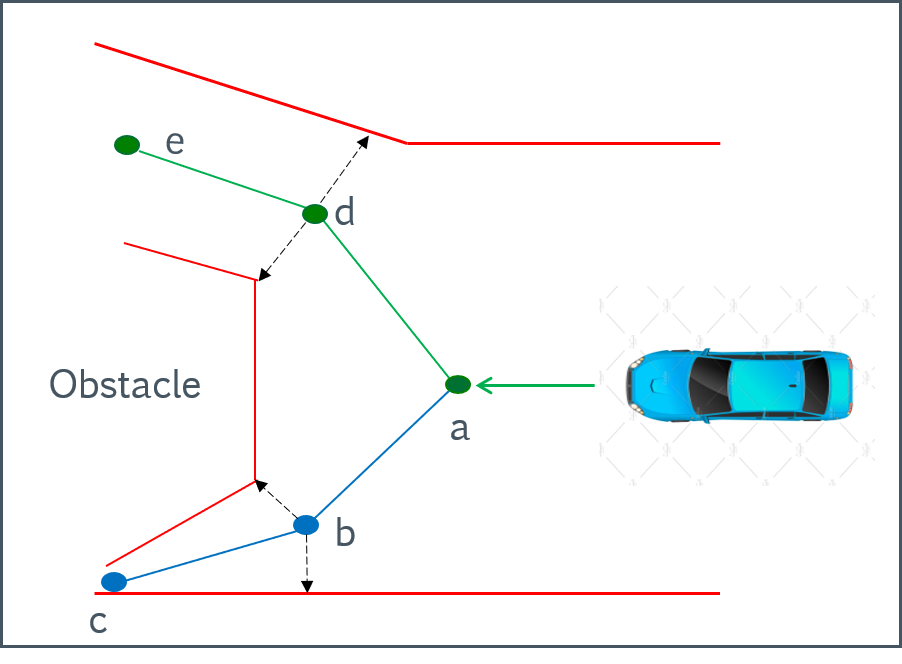
\includegraphics[width=2.5in]{Figures/rss_voronoi_plan.png}%
% \label{fig:voronoi_plan}%
% \caption{Constructing the roadmap from the Voronoi diagram for the given obstacles (in red). While safe roadmap ($<$\textbf{a}, \textbf{d}, \textbf{e}$>$) is highlighted in green, 
% Voronoi vertices, \textbf{b} and \textbf{c}, in the proximity of an obstacle are ignored during the roadmap construction. }
% \label{fig:vd_plan}
% \end{figure}



% \begin{figure}
% \centering
% \subfigure[]{%
% 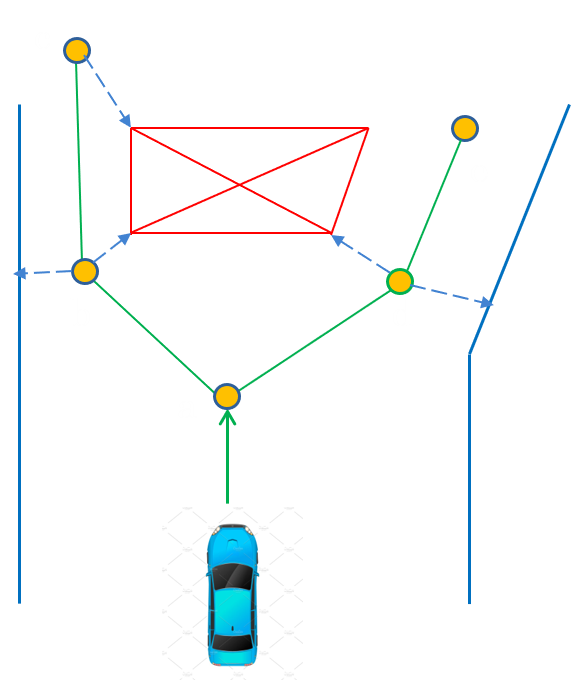
\includegraphics[width=1.6in]{Figures/vd_controller_1.png}%
% \label{fig:vd_contr_1}%
% }\qquad
% \subfigure[]{%
% 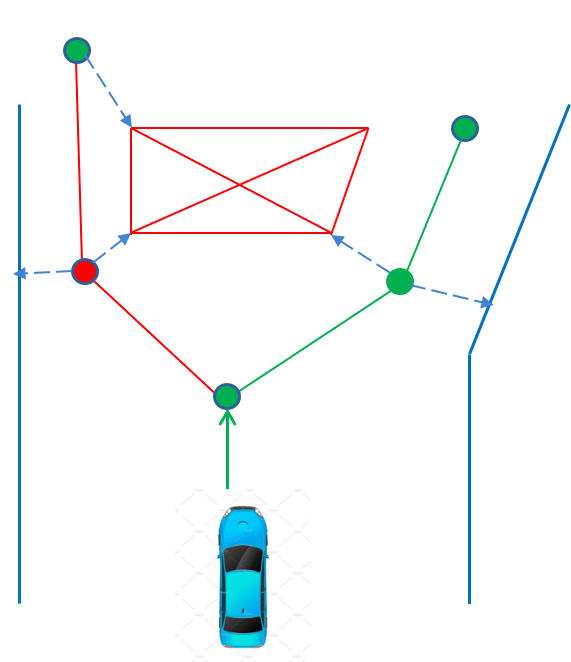
\includegraphics[width=1.6in]{Figures/vd_controller_2.png}%
% \label{fig:vd_contr_2}%
% }
% \caption{Constructing the roadmap from the Voronoi diagram.
% (a) shows the Voronoi diagram (in green) for the given walls and obstacles (in red).
% Some of the Voronoi vertices are close to the obstacle, so we ignore such vertices while constructing the roadmap.
% The corresponding roadmap is highlighted in green in (b). }
% \label{fig:vd_planner}
% \end{figure}

